%                                                                 aa.dem
% AA vers. 8.2, LaTeX class for Astronomy & Astrophysics
% demonstration file
%                                                       (c) EDP Sciences
%-----------------------------------------------------------------------
%
%\documentclass[referee]{aa} % for a referee version
%\documentclass[onecolumn]{aa} % for a paper on 1 column  
%\documentclass[longauth]{aa} % for the long lists of affiliations 
%\documentclass[rnote]{aa} % for the research notes
%\documentclass[letter]{aa} % for the letters 
%\documentclass[bibyear]{aa} % if the references are not structured 
% according to the author-year natbib style

%
%\documentclass[twocolumn]{aastex61}

\documentclass[%
 aip,
 twocolumn,
 jmp,%
 amsmath,amssymb,
%preprint,%
 reprint,%
%author-year,%
%author-numerical,%
]{aastex61}
\usepackage{amsmath}
\usepackage{graphicx}% Include figure files
\usepackage{dcolumn}% Align table columns on decimal point
\usepackage{bm}% bold math
\usepackage{relsize}
\usepackage{subfiles}

%\usepackage{aastex}

%\usepackage[mathlines]{lineno}% Enable numbering of text and display math
%\linenumbers\relax % Commence numbering lines
\newcommand{\Msun}{$M_{\odot}$}
\begin{document}

%\preprint{AIP/123-QED}

%\title[MEASURING DARK MATTER PROFILES NON-PARAMETRICALLY IN DWARF SPHEROIDALS]{MEASURING DARK MATTER PROFILES NON-PARAMETRICALLY IN DWARF SPHEROIDALS:
%	AN APPLICATION TO LEO I}% Force line breaks with \\
%\thanks{Footnote to title of article.}


%\date{\today}% It is always \today, today,
             %  but any date may be explicitly specified



%\pacs{Valid PACS appear here}% PACS, the Physics and Astronomy
                             % Classification Scheme.
%\keywords{Suggested keywords}%Use showkeys class option if keyword
                              %display desired



%\section{\label{sec:level1}}

\section{DATA}

\subsection{OBSERVATIONS}

This paper uses a large set of new radial velocity measurements taken within Leo I's half-light radius. The measurements were derived from spectra obtained with the Visible Integral-Field Replicable Unit Spectrograph, Wendelstein model (VIRUS-W) (Fabricius et al. 2008, 2012) mounted on the 2.7m Harlan J. Smith Telescope at McDonald Observatory in West Texas, using the instrument's high resolution mode; $R \sim 8600$ with wavelength coverage of 4855 \r{A} - 5475\r{A}. 

VIRUS-W is composed of 267 circular fibers. When mounted on the Harlan J. Smith Telescope, each fiber has a 3.2" diameter, with a total field-of-view of 105"  $\times$ 55" (wide side aligned east-west) and a 1/3 fill factor.

Two sets of observations were taken on December 2013 and January-February 2017 (hitherto referred as pointing 1 and pointings 2 and 3 respectively). Each exposure took either 3600s or 1800s with a total of 19 hours on pointing 1, 15 hours of pointing 2 and 7 hours of pointing 3. Seeing conditions ranged between 1.5" and 2.8", all below the fibers diameters. Sky spectra were taken from empty fibers. Calibration exposures for flats, bias and Hg-Ne arc lamp exposures were taken every night.
\begin{figure}
\centering
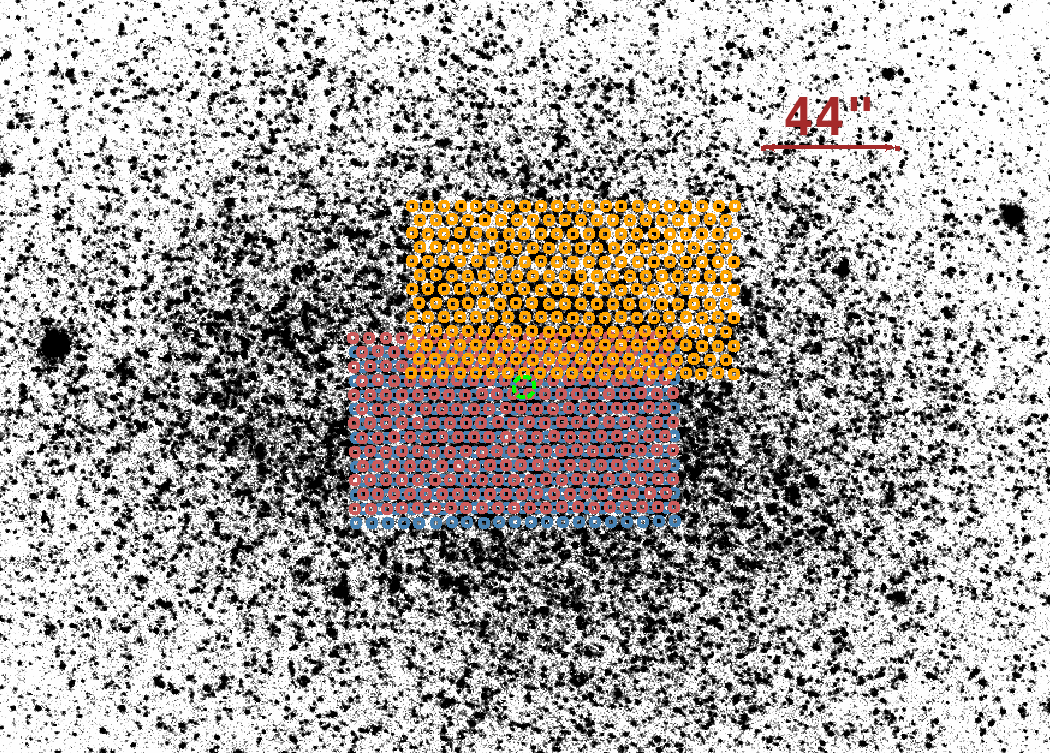
\includegraphics[width=0.5\textwidth]{pointing_inv.png}
\caption{The different spectral datasets taken with VIRUS-W. December 2013 (pointing 1) in orange and January-February 2017 (pointings 2 and 3) in red and blue. The photometric center of the galaxy is the green circle.}            
\end{figure}
    
\subsection{DATA REDUCTION}
\section{Observations and Data Reduction}


We use two sets of data for this paper.  We include new kinematic measurements obtained through the VIRUS-W instrument on the 2.7m telescope at McDonald Observatory.  We also include radial velocity measurements from Mateo et al. (2008).  Both datasets were obtained through integral field unit spectroscopy but differ in a few respects.  Mateo et al. (2008) targeted and obtained spectra for 328 bright, individual red giant branch (RGB) stars whose radii extend beyond the tidal radius of Leo I.  Our new observations are comprised of two pointings separated by $X”$ which target the inner radius of Leo I.  Due to the high stellar density in Leo I’s inner core, we use the integrated light of all fibers for our analysis rather than targeting single bright stars.  Figure X shows the radial distribution of our new measurements and that of Mateo et al. (2008). 


\subsection{VIRUS-W Observations and Data Reduction}


The VIRUS-W observations were carried out over X nights in January 2017 and Y nights in February 2017.  The conditions were mostly clear and were monitored using the guide star’s full width half maximum and photometric magnitude.  Each night we obtained twilight, Hg and Ne arc lamp, dome lamp, and bias exposures for calibration.  We employed an observing strategy which included two 3600s target exposures with two 1800s sky nod exposures, one before and one after.


We used a reduction software package called Panacea (https://github.com/grzeimann/Panacea), which is a general IFU reduction package used at McDonald Observatory.  Many of the routines employed in this package are similar to standard IFU reduction code but we describe them in detail here.  We began with the raw images and both subtracted and trimmed the overscan average value and region, respectively.  We constructed a single master bias frame over many nights and subtracted the resultant image from our science and twilight frames.  Using the twilight frames, we built a wavelength solution and a trace model for each of our fibers.  Twilights were taken at least once a night and typically in both the evening and morning.  As the ambient temperature changes, there are slight shifts in the trace of the fibers which are measureable in each of our science frames.  We use these derived shifts to correct our trace model for individual science frames and for the less illuminated 1800s sky frames we interpolated between the two closest science or twilight frames to get an adjusted trace model.  


The twilight frames also provide fiber profile measurements which overlap weakly ($<1\%$).  However, because of the overlap we solve for the one dimensional spectrum of each science and sky frame column by column solving the system of linear equations defined by:

\begin{align}

A\ x = b,

\end{align}

where $A$ is a matrix whose entries are the normalized fiber profile weights for the given column for each fiber, $b$ is the column of data from a given science or sky frame, and $x$ is the vector for which we solve which gives the spectrum for each fiber for the given column.  The spectral extraction is not done in rectified coordinates because the curvature of the trace is small enough that the error in not rectifying coordinates is less than $1\%$ for the whole CCD.


We use an iterative sky subtraction algorithm for our science observations as all fibers are filled with starlight from Leo I.  We first build master sky spectra from each sky frame.  We do this by applying an illumination model built from the twilight frame which corrects for fiber to fiber variations.  We then use time interpolated master sky spectra to first subtract sky from each science frame.  Coadding the individual science spectra for each of the two VIRUS-W pointings gives us a two master science models.  We subtract the master science spectra from the appropriate individual observations and use the resultant to build new master sky frames from the science subtracted science frames.  We iterate this procedure twice for convergence.  The final master sky models are subtracted from the individual science exposures and we coadd each pointing to get our final 534 fiber measurements.

\begin{comment}

Data reduction was performed using the VIRUS-W pipeline created by M. Fabricius, which itself is based on CURE, a data reduction software for the Hobby-Eberly Telescope Dark Energy Experiment (HETDEX), and the fitstools package (G{\"o}ssl \& Riffeser 2002).

The pipeline handles calibration, cosmic ray rejection, mapping and extraction of individual pixels to fiber number and wavelength, sky subtraction and combination into one final data "cube" (two spatial dimensions for the position of each fiber and one for the spectra).

Generically, the calibration process goes as follows: individual raw CCD files for every night are first converted into master bias, master flats and master arc frames. Bias subtracted master flats provide knowledge on throughput for normalization. Furthermore, their high flux helps clearly identify the position on which spectra from each individual fiber falls within the CCD.

In combination with master arcs, which help establish the position of known emission lines for wavelength calibration, their provide the distortion solution; a mapping from pixel positions on the CCD to their corresponding fiber number and wavelength.

With the calibration in hand, bias subtracted individual science frames are cleaned from cosmic rays via kappa-sigma clipping. Given the sparseness in between observations, heliocentric motion can present significant radial velocity variations (in our case of up to ~7 km/s within the same pointing). Hence, extraction of the individual frames takes each frame's date and time of exposure into account when correcting for its redshift due to heliocentric motion. This is done using a python implementation of Keck's heliocentric velocity calculation code (S. Burles \& D. Schlegel 2000). Finally, each frame's distortion solution and individual redshift get used to extract its spectra. The extracted spectra are subsequently corrected for throughput variations using the master flats.

%About 20\% of the fibers within the 2013 pointing landed on an empty field. Averaged together for each frame, flux from this fibers was removed from the rest to perform the sky subtraction.
The 2017 pointings presented almost no empty fibers. For this data sets, sky frames were taken between every couple of observations. Their reduction was done in the same fashion as their corresponding science frames but for the part in which the whole sky frame was subtracted from each adjacent science exposure.

Once the sky subtraction is done, all spectra for each individual pointing get combined on a final individual frame. The end product is a then a fully calibrated spectral cube.
To further specify the position and rotation of the spectral cube in the sky, an astrometry solution is derived from guider frames taken in parallel to the observations. The zero point between the guider field and the IFU field is calculated once per run. Finally, a data cube with flux on given RA,DEC and wavelength is created.
\end{comment}

\end{document}
